\documentclass{standalone}
\usepackage{tikz}
\usepackage{ctex,siunitx,upgreek}
\usepackage{tkz-euclide}
\usepackage{amsmath}
\usetikzlibrary{patterns, calc}
\usetikzlibrary {decorations.pathmorphing, decorations.pathreplacing, decorations.shapes,}
\begin{document}
\small
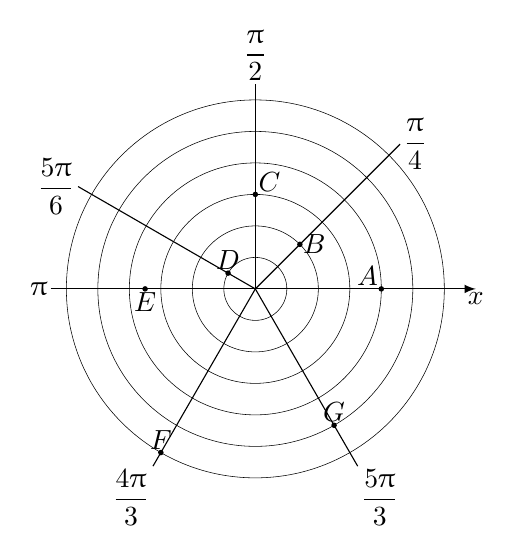
\begin{tikzpicture}[>=latex,scale=0.4,inner sep=1pt]
  % \tkzDefPoints{0/0/O,1/0/A}
  \draw[thin,->](-6.5,0)--(7,0)node[below]{$x$};
  % \draw[thin,->](0,-1.2)--(0,2.5)node[left]{$y$};
  \foreach \x/\t/\p [count=\i] in {45/{\dfrac{\uppi}{4}}/right,90/{\dfrac{\uppi}{2}}/above,150/{\dfrac{5\uppi}{6}}/left,180/{\uppi}/left,240/{\dfrac{4\uppi}{3}}/below left,300/{\dfrac{5\uppi}{3}}/below right} 
    { 
      \draw[very thin](0,0)circle(\i);
      \node at (\x:6.5)[\p]{$\t$}; 
    }
  \foreach \x/\y/\z/\p  in {0/4/A/above left,45/2/B/right,90/3/C/above right,150/1/D/above,180/3.5/E/below,240/6/F/above,300/5/G/above}
  {
    \draw(0,0)--(\x:6.5);
    \fill (\x:\y)circle(2.5pt)node[\p]{$\z$}; 
  }
\end{tikzpicture}
\end{document}